\documentclass{beamer}
\usepackage{polski}
\usepackage[utf8]{inputenc}
\usepackage{graphicx}

\usetheme{CambridgeUS}

\title{Ocena skuteczności i porównanie algorytmów dopasowania obrazów dla fotografii HDR}
\author[]{inż. Paweł Tobiszewski, \emph{179169}\\inż. Wojciech Majchrzyk, \emph{180791}}
\institute[PWr]{Politechnika Wrocławska, Wydział Informatyki i Zarządzania}

\begin{document}

\begin{frame}
	\titlepage
\end{frame}

%\begin{frame}
%	\frametitle{Agenda}
%	\tableofcontents
%\end{frame}

\begin{frame}
	\frametitle{Cel projektu}
	\begin{enumerate}
		\item Zapoznanie się z algorytmami tworzenia obrazow HDR
		\item Zaproponowanie metod porównania wyników działania algorytmów
		\item 
	\end{enumerate}
\end{frame}

\section{HDR}
\begin{frame}
	\frametitle{Co to jest HDR?}
	\begin{itemize}
		\item High Dynamic Range
		\item Ludzkie oko potrafi zarejestrować szeroki zakres jasności (od~$10^{-5}\frac{cd}{m^2}$~do~około~$10^9\frac{cd}{m^2}$)
		\item Aparaty fotograficzne nie są w stanie objąc całej tej skali jasności
		\item HDR polega na złączeniu ze sobą kilku fotografii wykonanych z różnymi parametrami
	\end{itemize}
\end{frame}

\begin{frame}
	\begin{figure}
		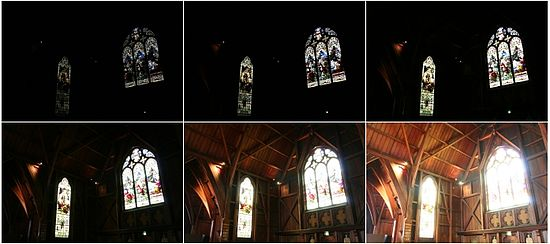
\includegraphics[height=.2\textheight]{res/images/HDRSources.jpg}
		\caption{Fotografie zrobione przy różnych parametrach przysłony}
	\end{figure}
	\begin{figure}
		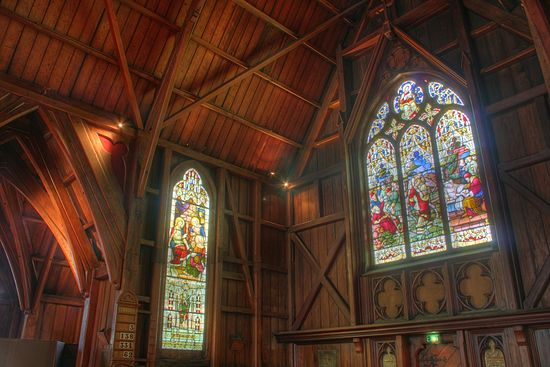
\includegraphics[height=.5\textheight]{res/images/HDRResult.jpg}
		\caption{Wynik - fotografia o szerszej dynamice tonalnej}
	\end{figure}
\end{frame}

\begin{frame}[allowframebreaks]
%	\begin{figure}
%		\includegraphics[width=\textwidth]{res/images/.jpg}
%	\end{frame}
\end{frame}

\begin{frame}
	\frametitle{Algorytmy HDR}
	Algorytmy do generowania zdjęć techniką HDR dostępne w pakiecie pfstools:
	\begin{enumerate}
		\item Fattal
		\item Drago
		\item Durand
		\item Mantiuk
	\end{enumerate}
	Do wykonania projektu użyjemy prawdopodobnie środowiska MatLAB~(Octave) oraz pakietu pfsTools.
\end{frame}

\begin{frame}
	\frametitle{Metody porównania algorytmów}
	\begin{itemize}
	\item Porównanie wyników działania poszczególnych algorytmów jest \textbf{mocno subiektywne}.
	\item Można stosować metody automatyczne, jak np. badanie wyrównania histogramu.
	\end{itemize}
\end{frame}

\end{document}
